\subsection{Enfoques de Valuaci\'on m\'as utilizados}

\begin{figure}[H]

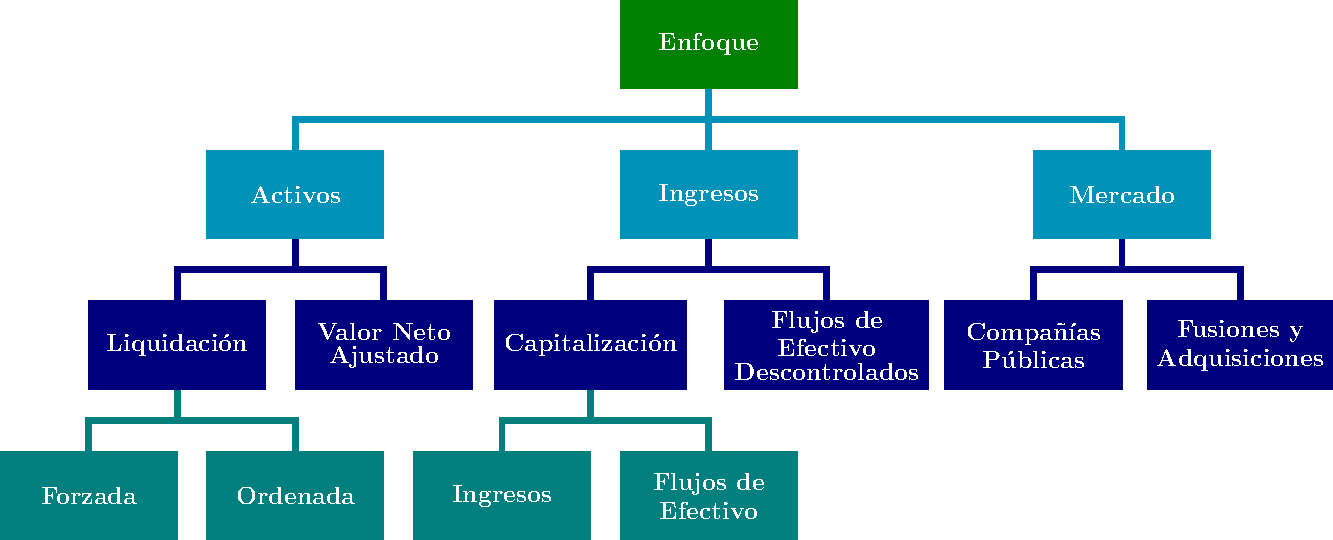
\includegraphics[width=7cm]{\rutaImagenes/enfoques_mas_utilizados}
      
\end{figure}

\tectcolor{principal}{\textbf{Enfoque de Activos.}} Este enfoque considera que el principal factor que determina el valor de una empresa es el valor de sus activos netos. Este enfoque es aplicable cuando no hay viabilidad del negocio en marcha y por tanto, se maximiza su valor en liquidación, o cuando el valor de un negocio yace en sus activos. 

\tectcolor{principal}{\textbf{Enfoque de Ingresos.}} Este enfoque asigna el valor de una compañía a su capacidad de generar flujos de efectivo y de obtener un retorno razonable sobre la inversión después de la consideración de los riesgos inherentes. El enfoque de ingresos incluye los métodos de ingresos o flujos capitalizados, así como de flujos descontados.

\tectcolor{principal}{\textbf{Enfoque de mercado.}} El enfoque empírico o de mercado consisten en determinar el valor de mercado de una compañía con base en el valor de razones o relaciones derivadas del análisis de los precios en transacciones de compañías públicas, aplicables a la empresa analizada. Tanto la información de fusiones y adquisiciones, así como la actividad de compraventa de acciones sirven para obtener medidas aplicables.

 